\documentclass[11pt,t]{beamer}
\usepackage{graphicx}
\graphicspath{{figures/}}
\usetheme{CambridgeUS}

\usepackage{mathtools}
\usepackage{array}

%Information to be included in the title page:
\title{BIOFLUID MECHANICS}
\subtitle{ON COMPUTATIONAL FLUID DYNAMICS}
\author{Vincent Belpaire}
\institute[]{Faculty of Architecture and Engineering\\Ugent}
\date{}

%Begin of section setup
\AtBeginSection[]
{
  \begin{frame}
    \frametitle{Table of Contents}
    \tableofcontents[currentsection]
  \end{frame}
}

\begin{document}
    
    \frame{\titlepage}

    \begin{frame}
        \frametitle{Table of Contents}
        \tableofcontents
    \end{frame}

    \section{Meshing}

    \begin{frame}
        \frametitle{The Aneurysm}
        \begin{figure}
            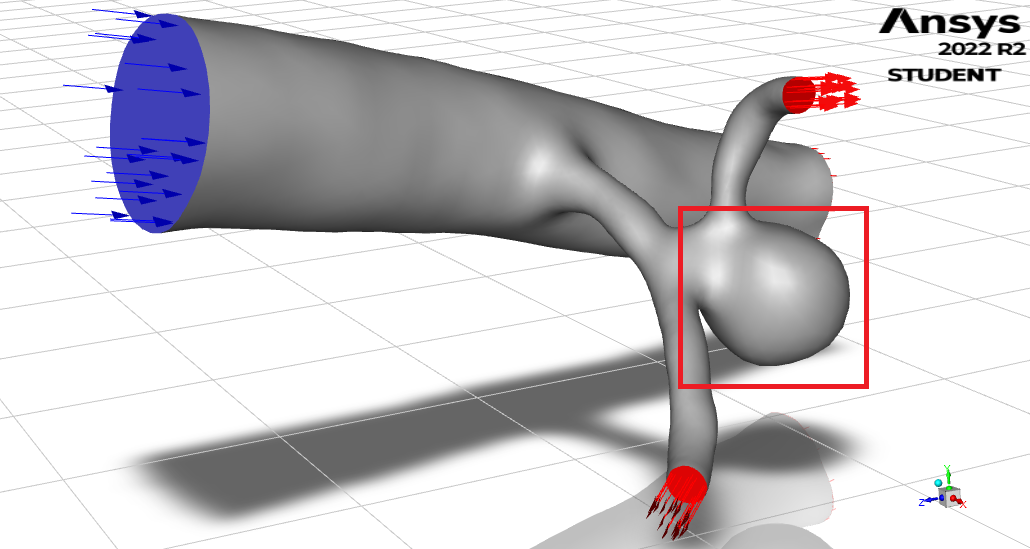
\includegraphics[width=\textwidth]{Mesh2_display1.png}
        \end{figure}
    \end{frame}

    \begin{frame}
        \frametitle{Mesh element types}
        \begin{figure}
            \centering
            \includegraphics<1>[width=0.45\textwidth]{Mesh2_edges_bulk.png}
            \includegraphics<1>[width=0.45\textwidth]{Mesh2_element_bulk.png}
            \includegraphics<2->[width=0.45\textwidth]{Mesh2_edges_boundary.png}
            \includegraphics<2->[width=0.45\textwidth]{Mesh2_element_boundary.png}
        \end{figure}
        \begin{minipage}{0.6\textwidth}
            \begin{itemize}
                \item[$\rightarrow$] in bulk tetrahedral (4 faces)
                \item<2->[$\rightarrow$] at boundaries prism 
            \end{itemize}
        \end{minipage}
        \begin{minipage}{0.3\textwidth}
            \includegraphics<-1>[width=0.5\textwidth]{tetr.png}
            \includegraphics<2->[width=0.5\textwidth]{prism.png}
        \end{minipage}
    \end{frame}

    \begin{frame}
        \frametitle{Mesh comparison}
        \begin{center}
            \begin{tabular}{m{0.2\textwidth} m{0.2\textwidth} m{0.2\textwidth} m{0.2\textwidth}}
                file & Element Type & $N$ & Bulk View\\
                Mesh1.cas & hexahedral, prism & 496718 & 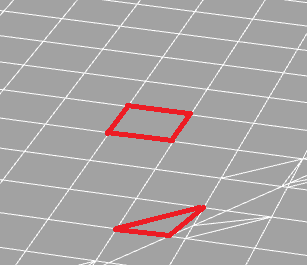
\includegraphics[width=0.15\textwidth]{Mesh1_element_bulk.png}\\
                Mesh2.cas & tetrahedral, prism & 80846 & 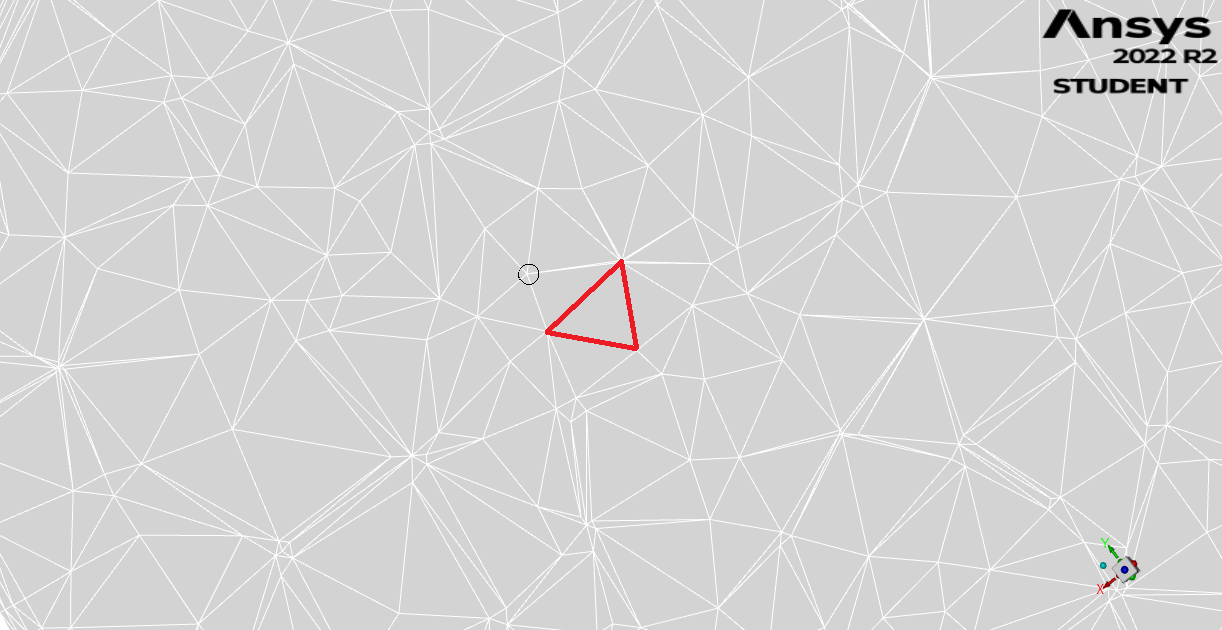
\includegraphics[width=0.15\textwidth]{Mesh2_element_bulk.png}\\
                Mesh3.cas & tetrahedral, prism & 319342 & 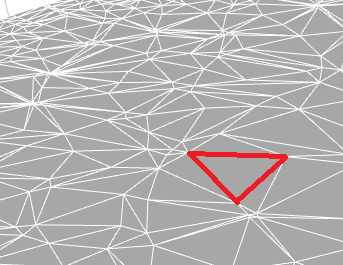
\includegraphics[width=0.15\textwidth]{Mesh3_element_bulk.png}\\
                Mesh4.cas & tetrahedral, prism & 486960 & 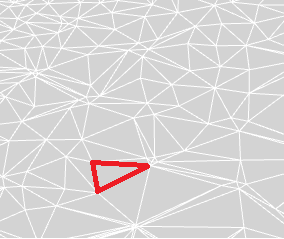
\includegraphics[width=0.15\textwidth]{Mesh4_element_bulk.png}
            \end{tabular} 
        \end{center}
    \end{frame}

    \section{Running an initial simulation}

    \begin{frame}
        \frametitle{Blood modelling}
        How is blood modelled by setting these values (density and viscosity) to be constant? Does this correspond to the normal behaviour of blood?
        \begin{itemize}
            \item<2->[$\rightarrow$] At large scales and relative high velocities, blood can be assumed to have a constant density (incompressible flow) and viscosity.
            \item<3->[$\rightarrow$] At small scales (around the size of a RBC) and relative slow velocities, blood can no longer be assumed homogeneous and it's apparent viscosity becomes very important.
            \item<4->[$\Rightarrow$]  This model is physiological.
        \end{itemize}
    \end{frame}

    \begin{frame}
        \frametitle{Results of initial simulation}
        \begin{itemize}
            \item<2->[$\rightarrow$] Mesh2 has the lowest number of elements $\Rightarrow$ Mesh2 is the coarsest mesh
            \item<3-> The residuals OK!
            \item<4-> Pressure contour: as expected, flow goes from higher pressures to lower pressures
            \item<5-> Conservation of mass?
        \end{itemize}
        \begin{center}
            \includegraphics<3>[width=0.7\textwidth]{Mesh2_residuals.png}
            \includegraphics<4>[width=0.7\textwidth]{Mesh2_pressure_contour.png}
            \begin{columns}
                \column<5->{0.4\textwidth}
                \begin{tabular}{c c}
                    Mass Flow Rate & [kg/s]\\ \hline
                    inlet.1.1 & 0.078264423\\
                    outlet-1.1.1 & -0.0039132212\\
                    outlet-2.1.1 & -0.0039132212\\
                    outlet-3.1.1 & -0.070437981\\ \hline
                    Net & -1.3877788e-17
                \end{tabular}
                \column<5->{0.4\textwidth}
                $\rightarrow$ Net mass flow rate $\approx 0$\\ $\Rightarrow$ mass is conserved!
            \end{columns}
        \end{center}
    \end{frame}

    \section{Mesh sensitivity analysis}

    \begin{frame}
        \frametitle{Mesh sensitivity}
        \begin{alertblock}<2->{Mesh sensitivity}
            Consider a quantity $A$ calculated via computational fluid dynamics with a mesh size $N$. Let's say that $A_1$ is calculated with a mesh size $N_1$ 
            and $A_2$ is calculated with a mesh size $N_2$, with $N_2 > N_1$. Then the mesh sensitivity, here denoted as $\epsilon$, between $A_1$ and $A_2$ is defined as 
            $$\epsilon = \frac{|A_2-A_1|}{N_2-N_1}=\frac{|\Delta{A}|}{\Delta{N}}.$$
        \end{alertblock}
        \begin{columns}
            \column<3->{\textwidth}
            $\epsilon$ indicates how much accuracy the model gains if the mesh size would be increase by $\Delta{N}$ elements. If $\epsilon$ is very small 
            and the computitional time relativly large then it would not be faivorable to increase the mesh size.
        \end{columns}
    \end{frame}

    \begin{frame}
            \begin{columns}
                \column{0.5\textwidth}
                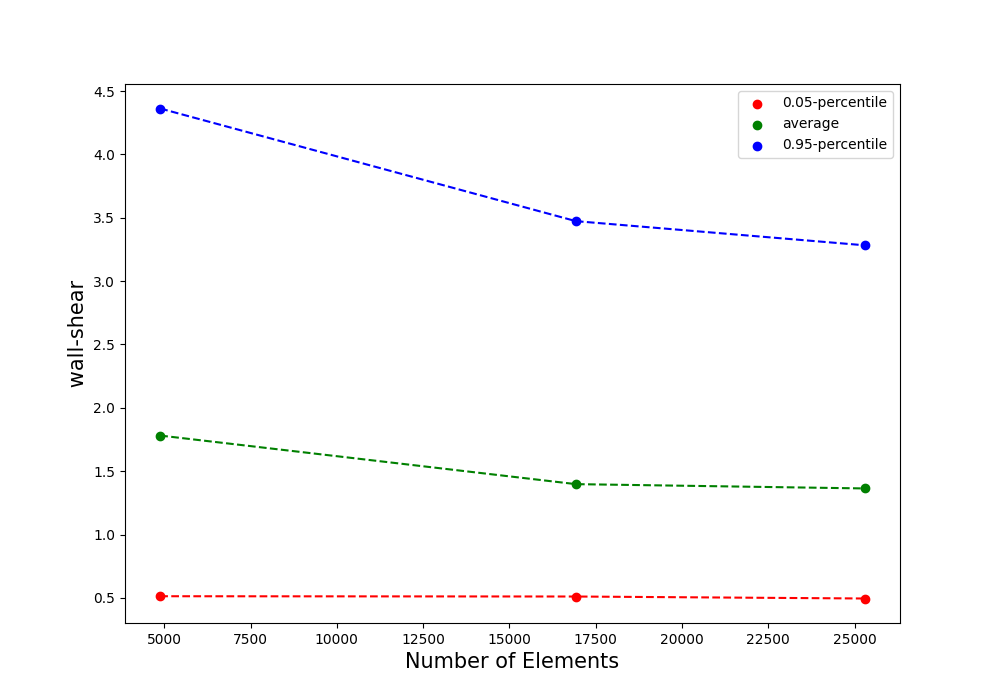
\includegraphics[width=\textwidth]{wall-shear_MSA.png}
                \column{0.5\textwidth}
                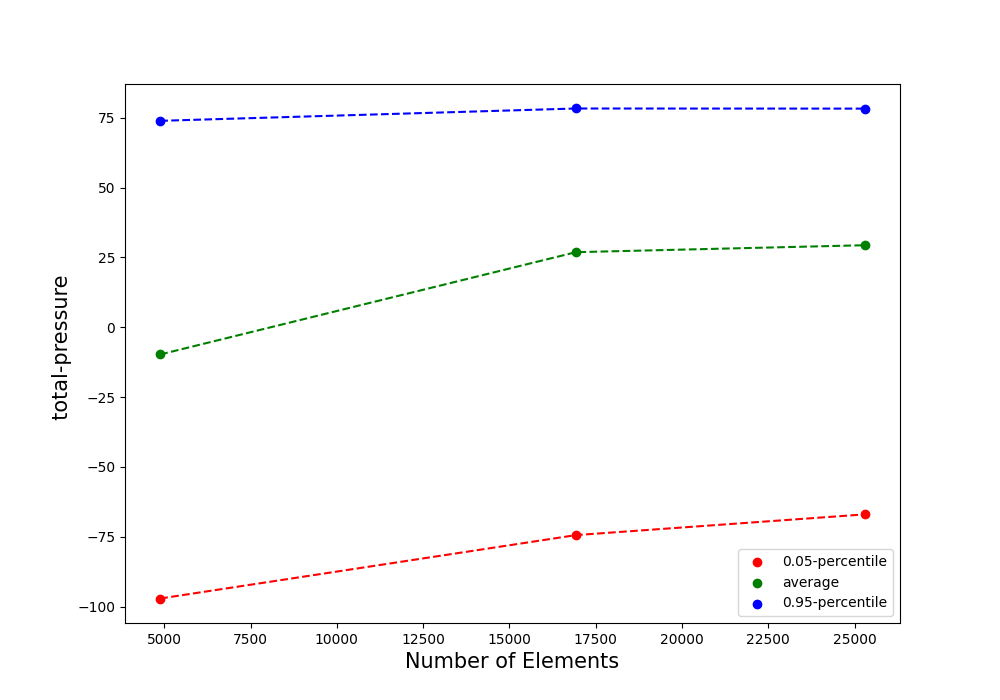
\includegraphics[width=\textwidth]{total-pressure_MSA.png}
            \end{columns}
        \begin{itemize}
            \item<2->[] Observations:
            \item<3->[$\rightarrow$] From Coarse to Medium: relative high improvement
            \item<4->[$\rightarrow$] \alert<6->{From Medium to Fine: relative low improvement}
            \item<5->[$\rightarrow$] Estimate computation time (all \alert{converged}!): 
            \item<5->[] Coarse: $T$ $<$ 3 min
            \item<5->[] \alert<6->{Medium: 2 min $<$ $T$ $<$ 4 min }
            \item<5->[] Fine: 5 min $<$ $T$
            \item<7->[$\Rightarrow$] Medium mesh will suffice
        \end{itemize}
    \end{frame}

    \begin{frame}
        \frametitle{Reflection}
        \begin{itemize}
            \item<2-> Why usage of percentiles and not minimum or maximum?
            \item<3->[$\rightarrow$] preventing outliers to influence conclusion
            \item<4-> More advanced techniques for mesh sensitivity analysis?
            \item<5->[$\rightarrow$] Numerical Mathematics: knowing the structure of the CFD model and its properties
        \end{itemize}
    \end{frame}

    \begin{frame}
        \begin{center}
            
\includegraphics[width=\textwidth]{IMG_3565.jpg}    
        \end{center}
    \end{frame}

\end{document}